% Completa los datos convenientemente en las zonas marcadas con TODO

\documentclass{beamer}
%PARA VISUALIZAR PRESENTACIONN CON NOTAS USAR VISUALIZADOR "pdfpc":
%Para ver las notas, el cronometro y siguente diapo:
% pdfpc --notes=right slides.pdf
% "tecla p": para pausar el cronometro
\mode<presentation> {
  \usetheme{CambridgeUS}
  \usecolortheme{crane} % color naranja
}
\setbeamercolor{titlelike}{parent=structure,bg=yellow!85!orange} % Cambia el color de la caja del título de la página inicial

\setbeamertemplate{navigation symbols}{} % ocultar iconos de navegación
\setbeamerfont{subsection in toc}{size=\small} % reducir tamaño en TOC
\setbeamerfont{date}{size=\tiny}
\usepackage[spanish]{babel}
\usepackage[utf8]{inputenc}
\usepackage{graphicx}
\usepackage{booktabs}
\usepackage{hyperref}
\usepackage{multicol}
\usepackage{pgfpages}
\usepackage{listings}
\usepackage{multimedia}
\usepackage[export]{adjustbox}
\usepackage{outlines} % Para poner bullets tabulados (\1 \2 \3 ...) y no items
\usepackage{fontawesome5} 
\usepackage{array,tabularx} % para tabular leyenda de ecuaciones
\newenvironment{conditions*} % entorno de "leyenda de ecuación"
  {\par\vspace{\abovedisplayskip}\noindent
   \tabularx{\columnwidth}{>{$}l<{$} @{\ : } >{\raggedright\arraybackslash}X}}
  {\endtabularx\par\vspace{\belowdisplayskip}}
  
% USO DE NOTAS
\setbeameroption{hide notes} % Para mostrar u ocultar (hide/show)
%\setbeameroption{show only notes} % Mostrar solo las notas
%\setbeameroption{show notes on second screen=right} % Mostrar notas en otra pantalla
\setbeamertemplate{note page}{ % asi solo muestro el texto de las notas
  \insertnote%
}

%========= TODO: datos internos del documento
\hypersetup{
	pdftitle={Defensa de trabajo de fin de grado de Pon tu nombre},
	pdfauthor={Pon tu nombre},
	pdfsubject={Pon aquí el título completo del trabajo},
	pdfkeywords={teaching, robotics, vision, sensors, actuators, raspberry},
	pdfproducer={pdfLaTeX},
  colorlinks=true,
  linkcolor=blue
}
%=========

%========= TODO: diapositiva de portada
\title[Robot de bajo coste guiado por voz]{Prototipo de robot de bajo coste guiado por voz con técnicas de localización} % El título reducido aparece en la parte inferior de todas las diapositivas
                                         % El título completo aparece solo en la diapositiva de portada
\author[Víctor de la Torre Rosa]{Víctor de la Torre Rosa}
\institute[URJC]
{
\textit{\href{mailto:escribe.tu@correo.es}{\color{blue}{\underline{v.delatorre.2019@alumnos.urjc.es}}}}\\
\vspace{0.5cm}

\includegraphics[width=3cm]{figs/logo-urjc}\\
\vspace{1cm}
Trabajo Fin de Grado
}
\date{18 de marzo de 2025}
%=========

%========= COMIENZO DEL DOCUMENTO
\begin{document}

%========= Portada inicial con notas
\begin{frame}[plain] % plain: quita header y footer
\large{\titlepage}
\note[item]{En esta presentación voy a hablar sobre...}
\note[item]{En primer lugar...}
\end{frame}

%========= Licencia
\begin{frame}
% Este diseño se corresponde con la licencia CC-BY-NC-SA.
% Por supuesto, puedes poner la licencia que mejor se adapte al propósito de tu trabajo.
% Recuerda que, si no se especifica ninguna licencia, esta -como cualquier creación artística- pasaría a estar licenciada con todos los derechos reservados (copyright).

\cleardoublepage

\begin{flushright}
\begin{figure}
 \ \ \ \ 
\includegraphics[width=0.25\linewidth,right]{figs/by-sa.png}
 \label{fig:cc} 
 \end{figure}
\end{flushright}

\

\

\

\noindent
Este trabajo se distribuye bajo los términos de la licencia internacional \href{http://creativecommons.org/licenses/by-sa/4.0/}{CC BY-SA International License} (Creative Commons Attribution-ShareAlike 4.0). Usted es libre de \textit{(a) compartir}: copiar y redistribuir el material en cualquier medio o formato para cualquier propósito, incluso comercialmente; y \textit{(b) adaptar}: remezclar, transformar y construir a partir del material para cualquier propósito, incluso comercialmente. La licenciante no puede revocar estas libertades en tanto usted siga los términos de la licencia:

\begin{itemize}
\item \textit{Atribución}. Usted debe dar \href{https://creativecommons.org/licenses/by-sa/4.0/deed.es#ref-appropriate-credit}{crédito de manera adecuada}, brindar un enlace a la licencia, e indicar \href{https://creativecommons.org/licenses/by-sa/4.0/deed.es#ref-indicate-changes}{si se han realizado cambios}. Puede hacerlo en cualquier forma razonable, pero no de forma tal que sugiera que usted o su uso tienen el apoyo de la licenciante.
\item \textit{Compartir igual}. Si remezcla, transforma o crea a partir del material, debe distribuir su contribución bajo la \href{https://creativecommons.org/licenses/by-sa/4.0/deed.es#ref-same-license}{misma licencia} del original.\\
No hay restricciones adicionales — No puede aplicar términos legales ni \href{https://creativecommons.org/licenses/by-sa/4.0/deed.es#ref-technological-measures}{medidas tecnológicas} que restrinjan legalmente a otras a hacer cualquier uso permitido por la licencia.
\end{itemize}

\begin{flushright}
		\vspace{7.0 cm}
		\emph{Documento de} \textbf{Víctor de la Torre Rosa}. % TODO: pon aquí tu nombre cuando hagas el documento
\end{flushright}


\end{frame}

%========= Índice o tabla de contenidos (TOC)
\begin{frame}
\frametitle{Contenidos}
\begin{multicols}{2} % si tengo muchas secciones, lo parte en dos columnas
  \tableofcontents[hideallsubsections] % no muestra subsecciones
\end{multicols}
\note[item]{La presentaci\'on esta dividida en cuatro partes.}
\end{frame}

%========= Diapositiva "vacía" de comienzo de sección:
\section*{}
\begin{frame}{}
  \centering \Huge
  \emph{Introducción}
\note[item]{Comencemos con la introducción.}
\end{frame}

\section{Introducción}
\subsection{Contexto general}
%========= Diapositiva con imágenes:
\begin{frame}
\frametitle{Robótica móvil}
\centering
\begin{minipage}{0.45\textwidth}
    \centering
    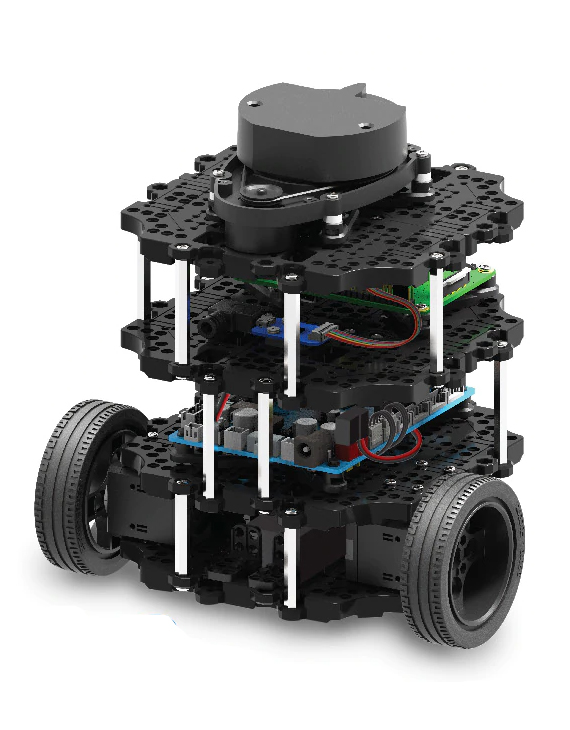
\includegraphics[width=3.4cm]{figs/turtlebot3burguer.jpg}
\end{minipage}
\hfill
\begin{minipage}{0.45\textwidth}
    \centering
    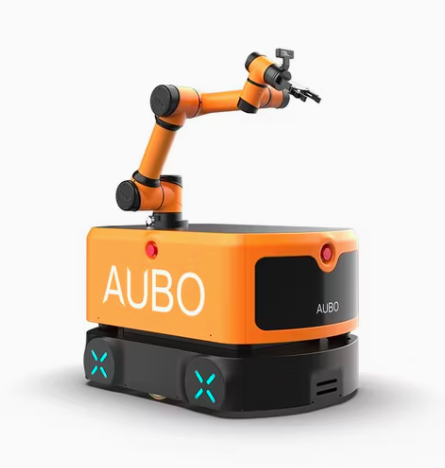
\includegraphics[width=3.4cm]{figs/ttt.png}
\end{minipage}
\end{frame}





%========= Diapositiva con ítems resaltados con colores:
\begin{frame}
\frametitle{Robótica educativa y de bajo coste}
\centering

% Primera fila
\begin{minipage}{0.45\textwidth}
    \centering
    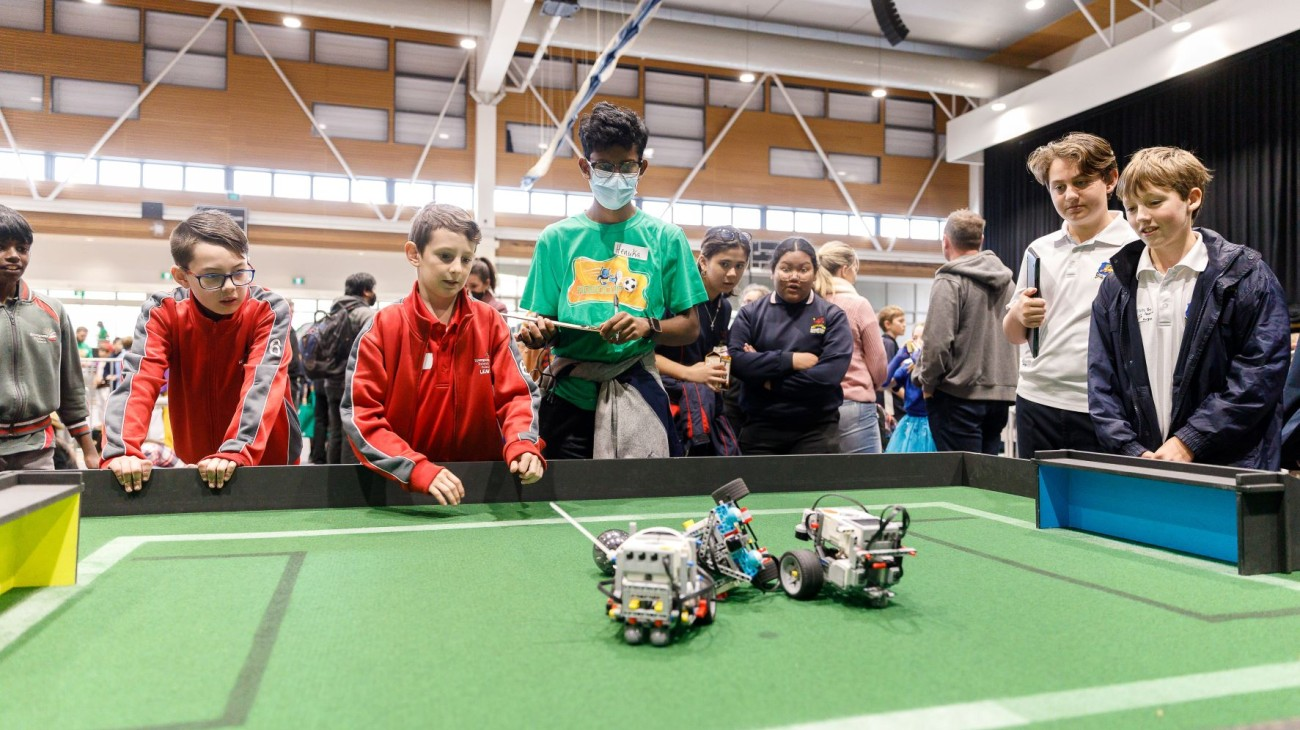
\includegraphics[width=3.4cm]{figs/RoboCup_junior.jpg}
\end{minipage}
\hfill
\begin{minipage}{0.45\textwidth}
    \centering
    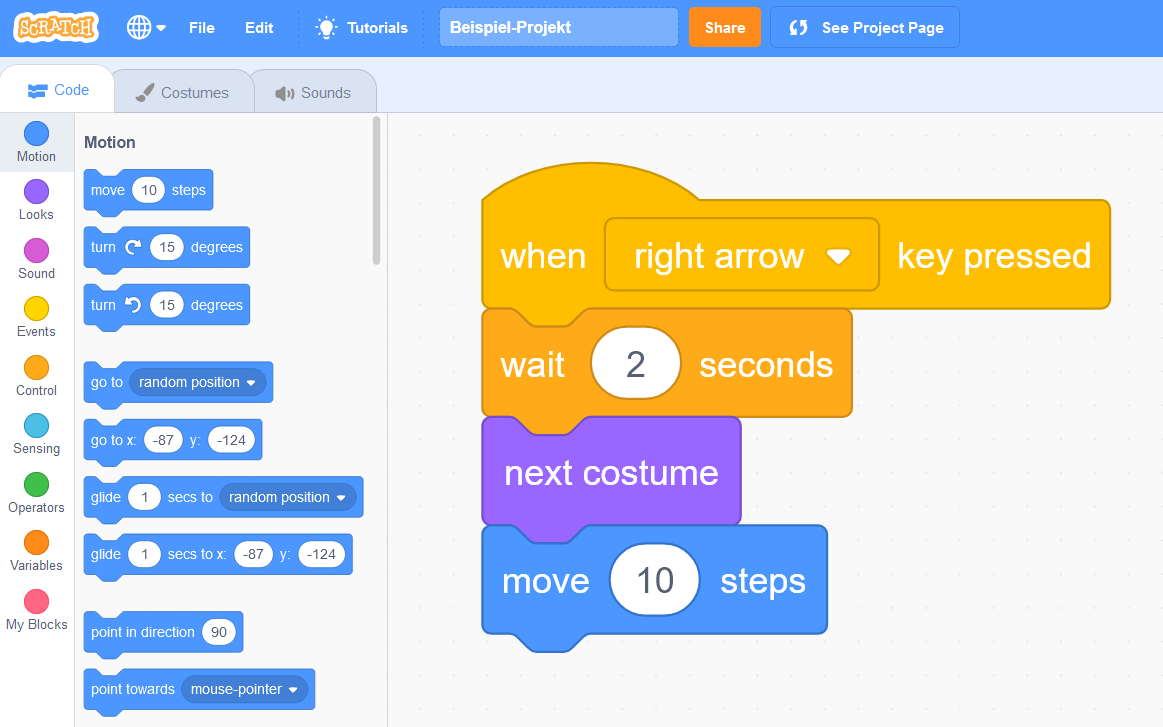
\includegraphics[width=3.4cm]{figs/scratch.png}
\end{minipage}

\vspace{0.5cm} % Espacio entre filas

% Segunda fila
\begin{minipage}{0.45\textwidth}
    \centering
    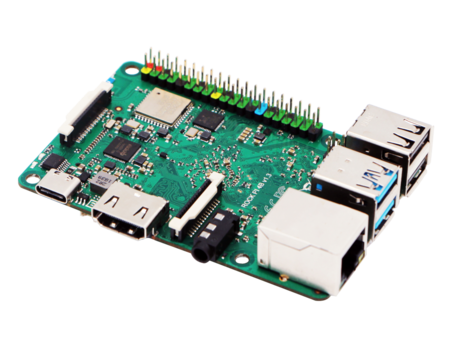
\includegraphics[width=3.4cm]{figs/raspberry4.png} % Cambia por la ruta de la tercera imagen
\end{minipage}
\hfill
\begin{minipage}{0.45\textwidth}
    \centering
    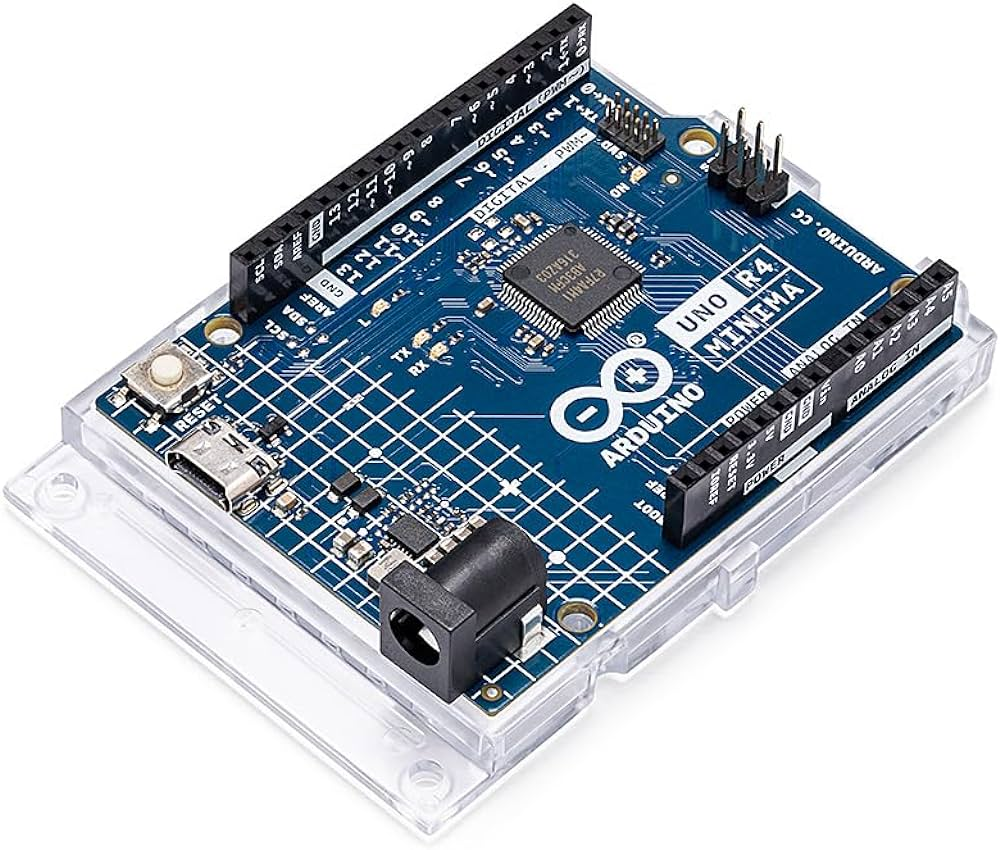
\includegraphics[width=3.4cm]{figs/arduino_uno.jpg} % Cambia por la ruta de la cuarta imagen
\end{minipage}

\end{frame}



\section*{}
\begin{frame}{}
  \centering \Huge
  \emph{Objetivos}
\note[item]{Pasemos ahora a comentar los objetivos que nos hemos con este trabajo.}
\end{frame}

\section{Objetivos}
\begin{frame}
\frametitle{Descripción del problema}
\centering

% Primera fila
\begin{minipage}{0.45\textwidth}
    \centering
    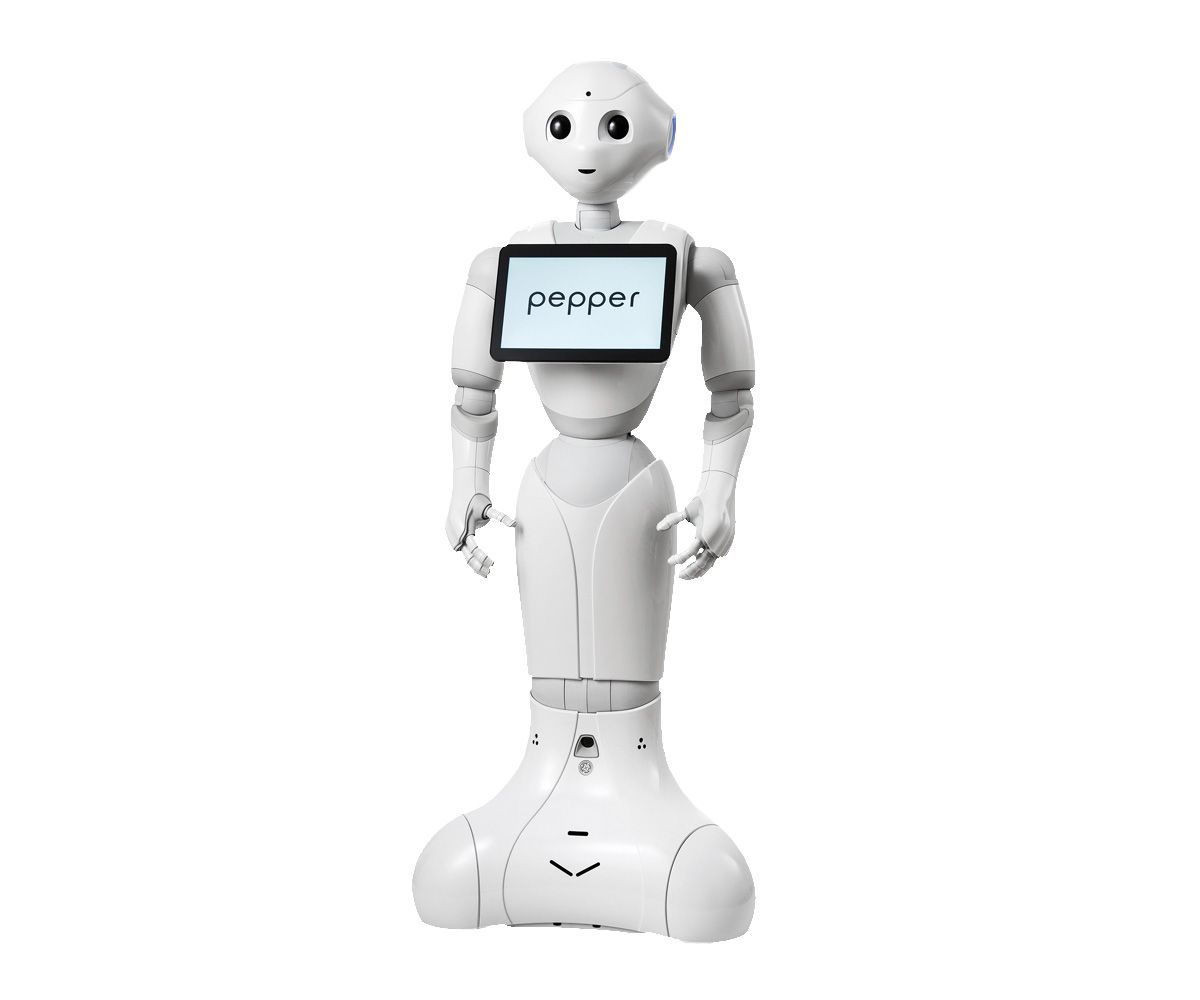
\includegraphics[width=4.4cm]{figs/peper.jpg}
\end{minipage}
\hfill
\begin{minipage}{0.45\textwidth}
    \centering
    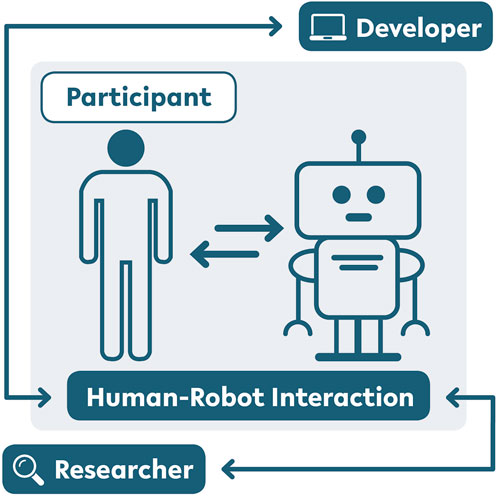
\includegraphics[width=3.8cm]{figs/hri.jpg}
\end{minipage}

\vspace{0.5cm} % Espacio entre filas

% Segunda fila
\begin{minipage}{0.45\textwidth}
    \centering
    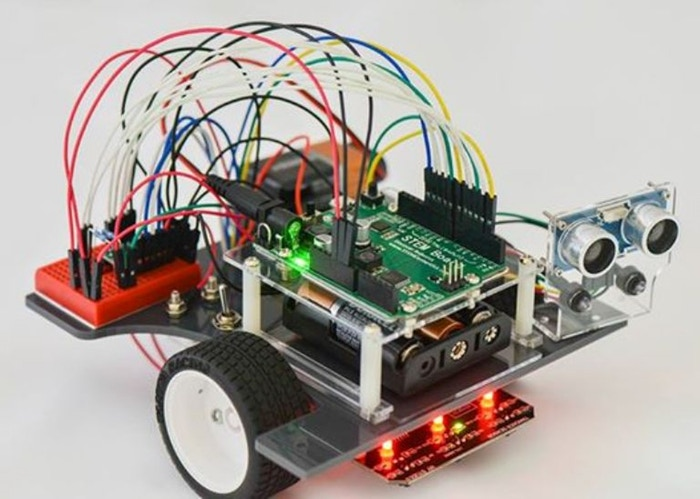
\includegraphics[width=3.8cm]{figs/robot_rasp.jpg} % Cambia por la ruta de la tercera imagen
\end{minipage}
\hfill
\begin{minipage}{0.45\textwidth}
    \centering
    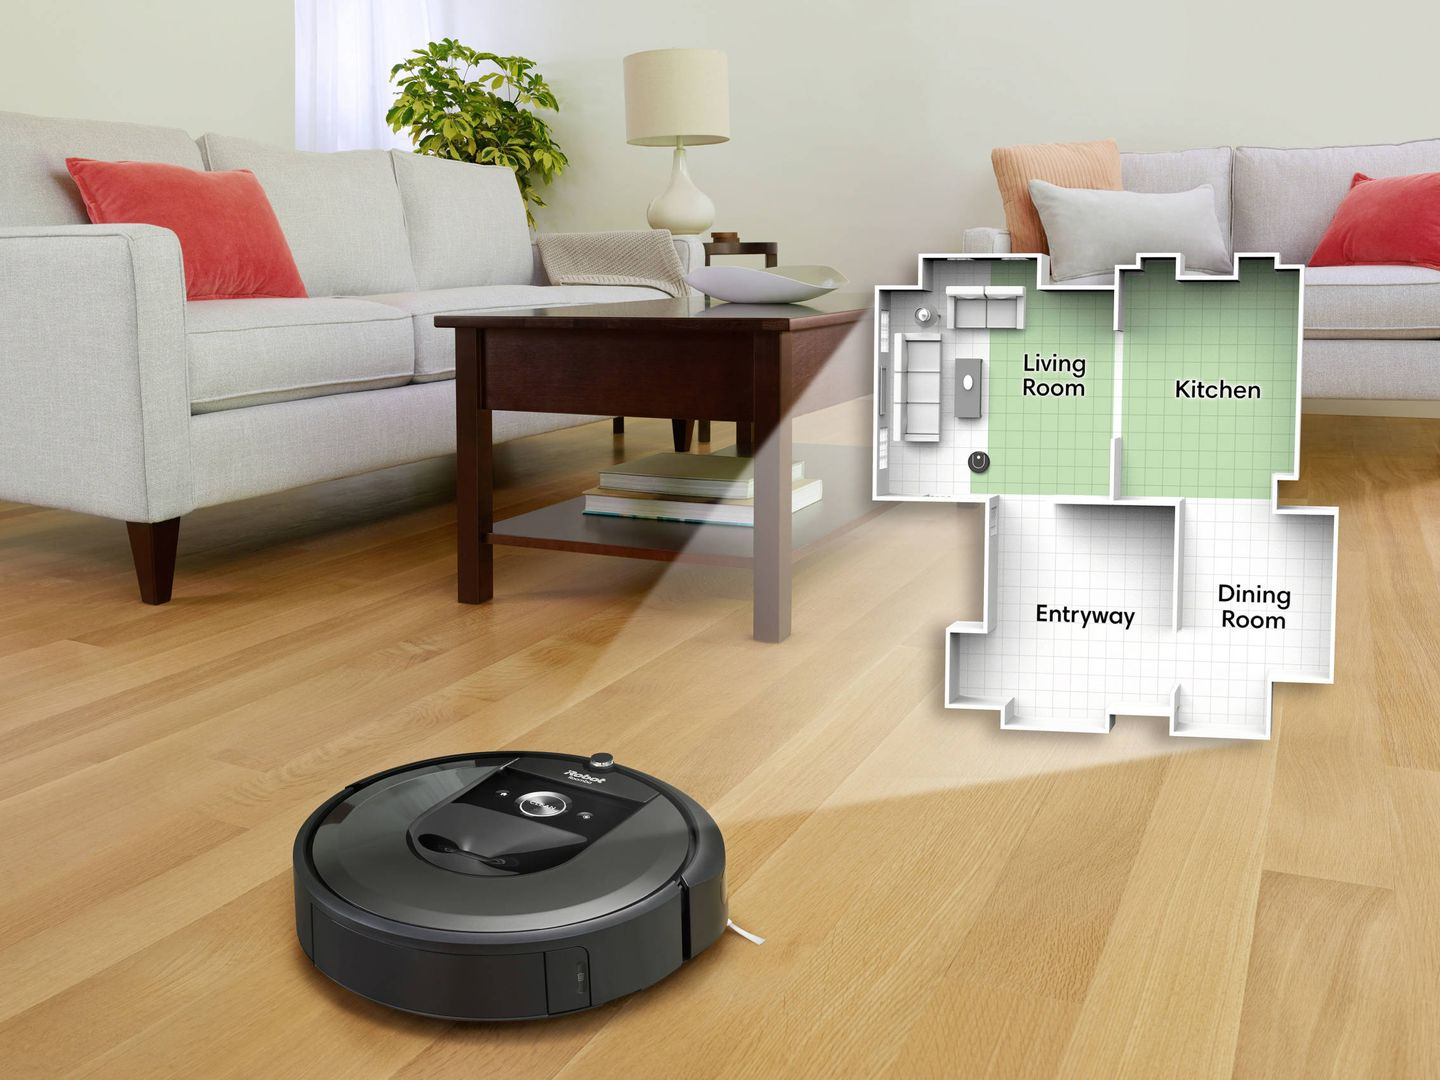
\includegraphics[width=3.8cm]{figs/rumba.jpg} % Cambia por la ruta de la cuarta imagen
\end{minipage}

\end{frame}


\begin{frame}
\frametitle{Requisitos}
\begin{enumerate}
    \item 145€.
    \item \faDollarSign
    \item \faWifi % Ícono de Wi-Fi en lugar de texto
    \item Impresora convencional 3D.
    \item Tiempo real.
    \item Python.
    \item Batería recargable.
    \item Peso ligero.
\end{enumerate}
\end{frame}

\begin{frame}
\frametitle{Objetivos específicos}
\begin{enumerate}
\item Diseño.
\item Estado del arte.
\item Control del robot.
\item Navegación + Localización.
\item Calibración.
\item Red neuronal.
\end{enumerate}
\end{frame}

\begin{frame}
\frametitle{Metodología}
\centering
\begin{minipage}{0.45\textwidth}
    \centering
    
\includegraphics[width=5.4cm]{figs/git.png}
\end{minipage}
\hfill
\begin{minipage}{0.45\textwidth}
    \centering
    
\includegraphics[width=3.2cm]{figs/teams.png}
\end{minipage}
\vfill

\href{https://github.com/RoboticsURJC/tfg-vdelatorre}{https://github.com/RoboticsURJC/tfg-vdelatorre}
\end{frame}

\section*{}
\begin{frame}{}
  \centering \Huge
  \emph{Plataforma de desarrollo}
\note[item]{Una vez descritos los objetivos, veamos qué hemos hecho para alcanzarlos.}
\end{frame}


\section{Plataforma de desarrollo}
\begin{frame}
\frametitle{Hardware}
\centering

% Primera fila
\begin{minipage}{0.3\textwidth}
    \centering
    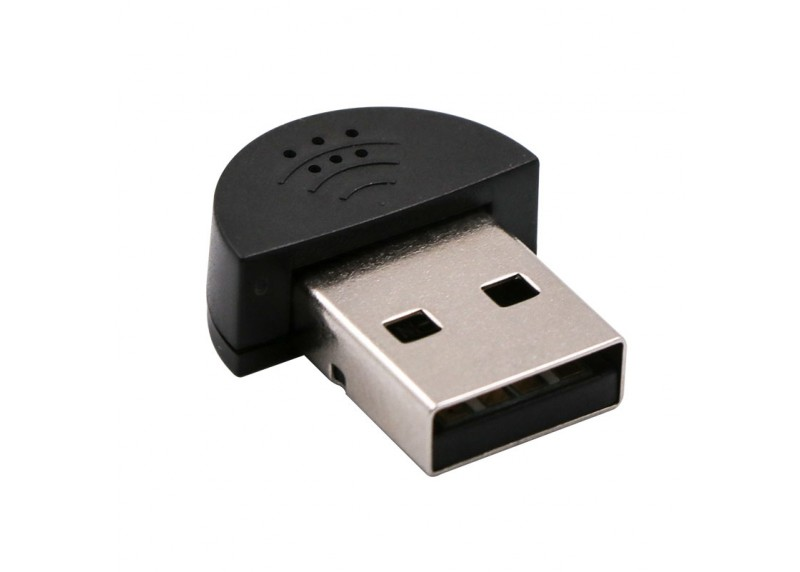
\includegraphics[width=2.3cm]{figs/microfono-usb.jpg}
\end{minipage}
\hfill
\begin{minipage}{0.3\textwidth}
    \centering
    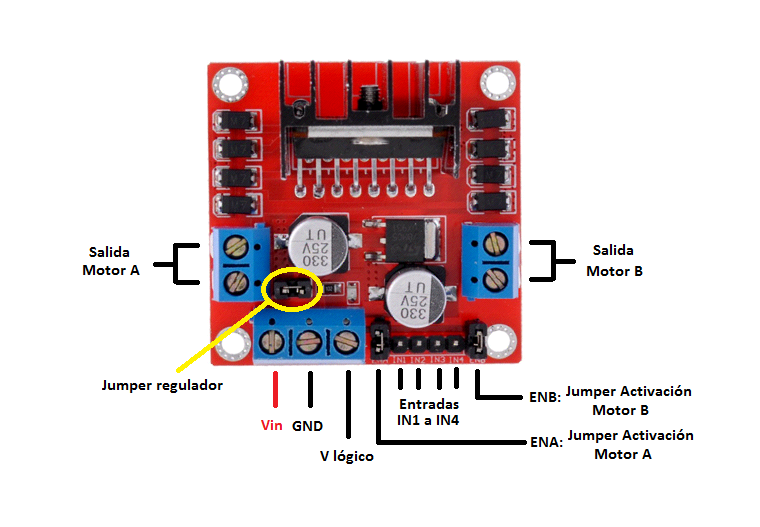
\includegraphics[width=3.0cm]{figs/L298N.png}
\end{minipage}
\hfill
\begin{minipage}{0.3\textwidth}
    \centering
    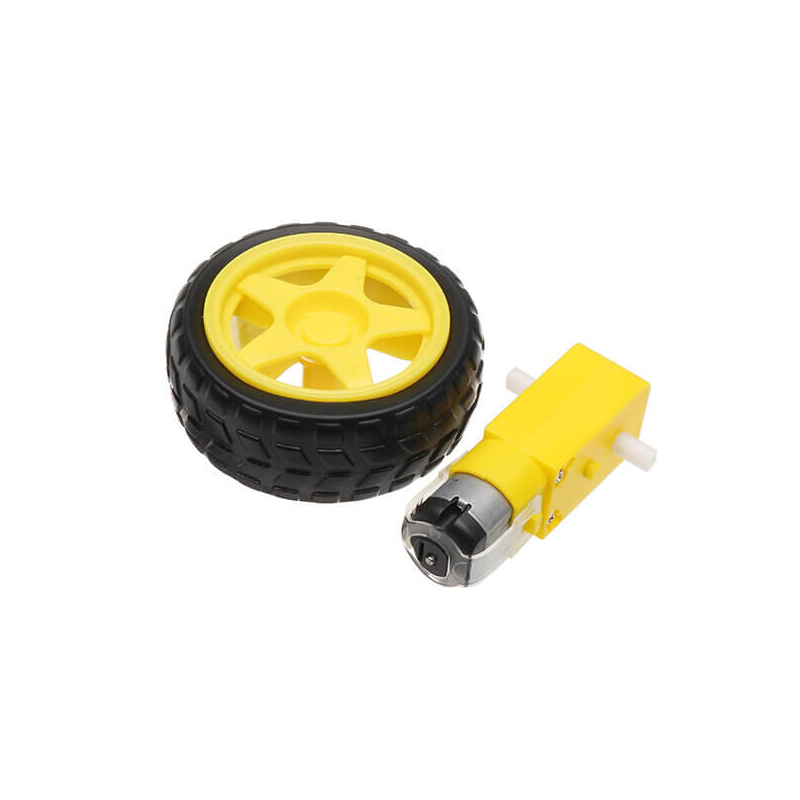
\includegraphics[width=2.6cm]{figs/motor.jpg}
\end{minipage}

\vspace{-0.3cm} % Reduce el espacio entre filas


% Segunda fila
\begin{minipage}{0.3\textwidth}
    \centering
    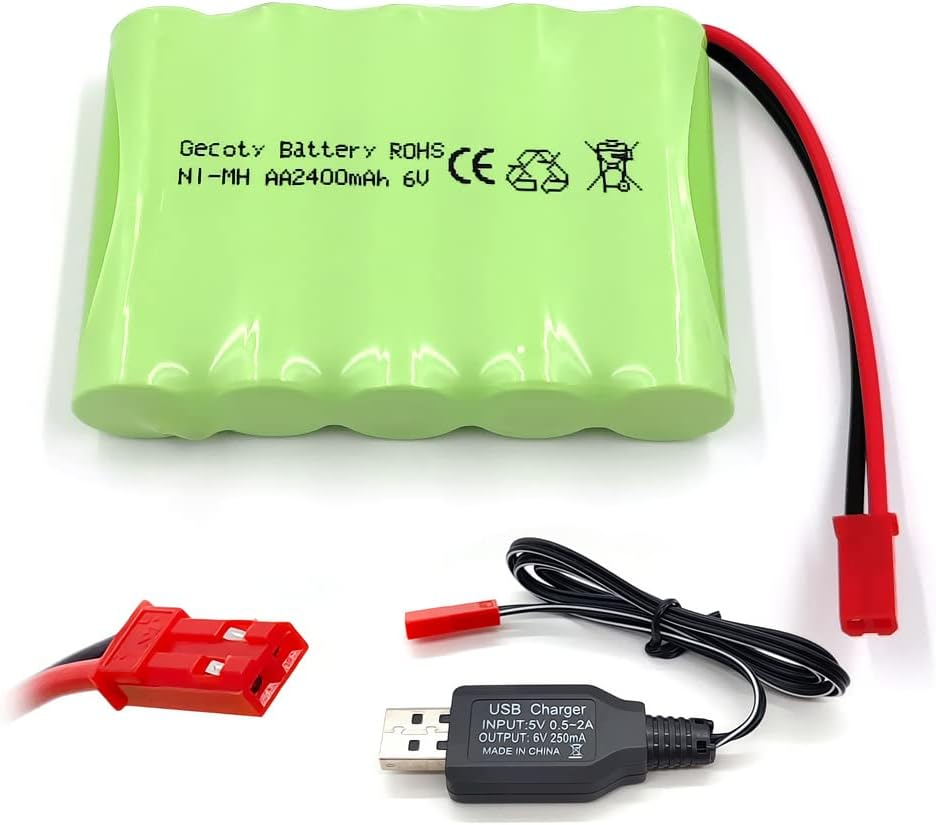
\includegraphics[width=2.0cm]{figs/bateria.jpg} 
\end{minipage}
\hfill
\begin{minipage}{0.3\textwidth}
    \centering
    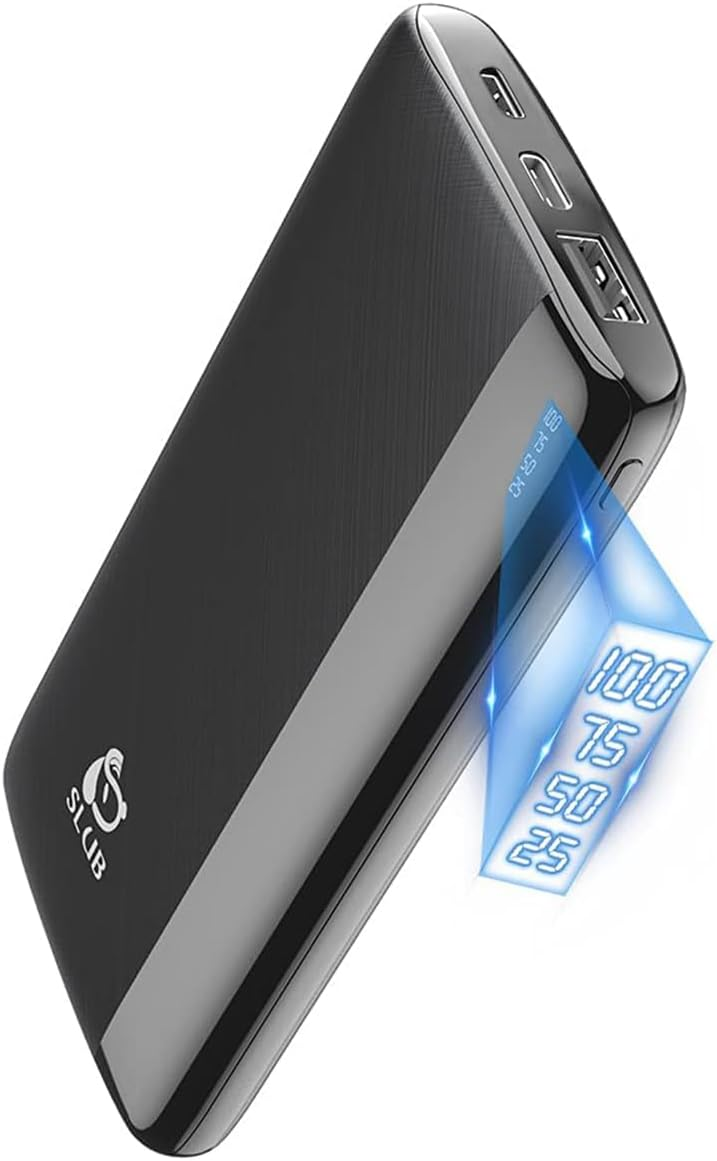
\includegraphics[width=1.1cm]{figs/powerbank.jpg} 
\end{minipage}
\hfill
\begin{minipage}{0.3\textwidth}
    \centering
    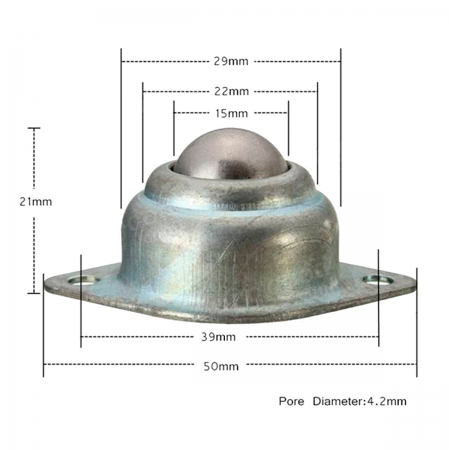
\includegraphics[width=2.0cm]{figs/rueda_loca.png}
\end{minipage}



% Tercera fila
\begin{minipage}{0.3\textwidth}
    \centering
    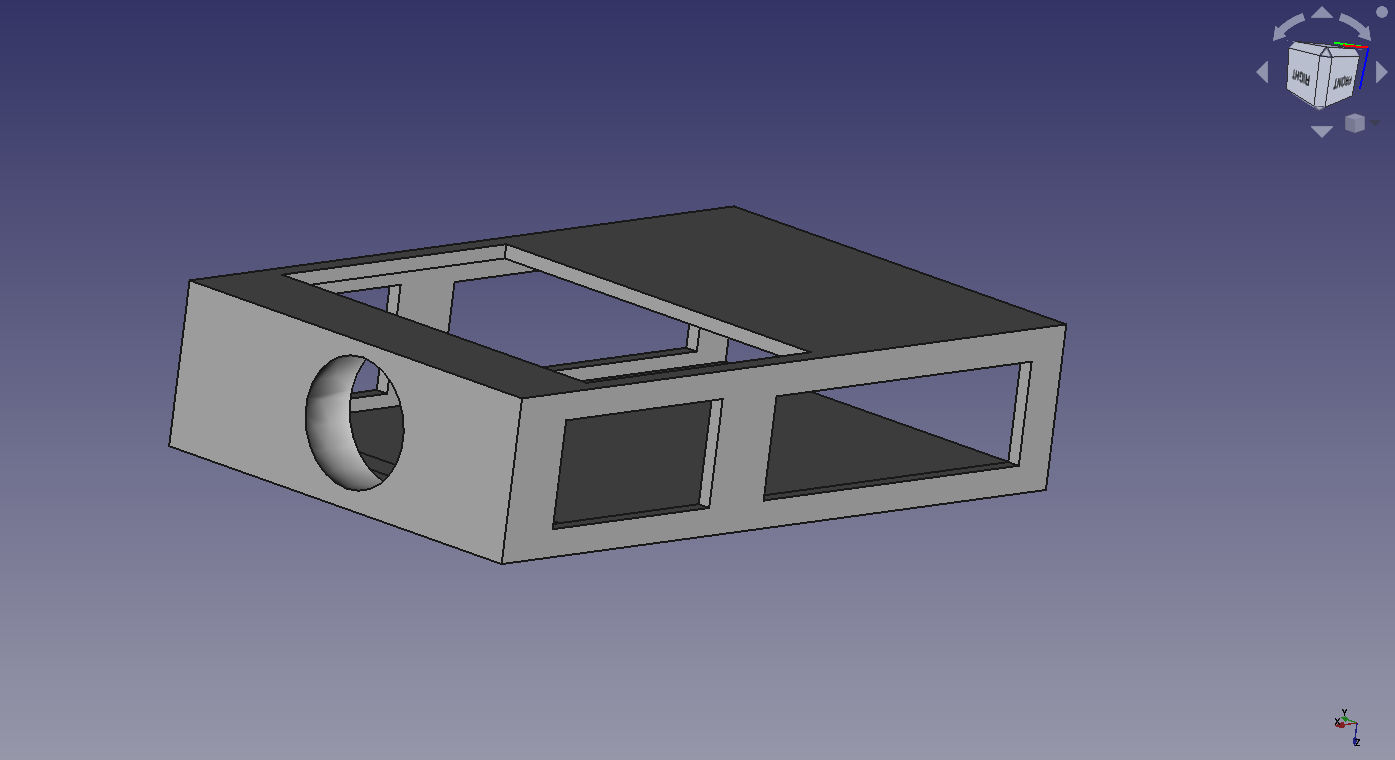
\includegraphics[width=3.5cm]{figs/base.png} 
\end{minipage}
\hfill
\begin{minipage}{0.3\textwidth}
    \centering
    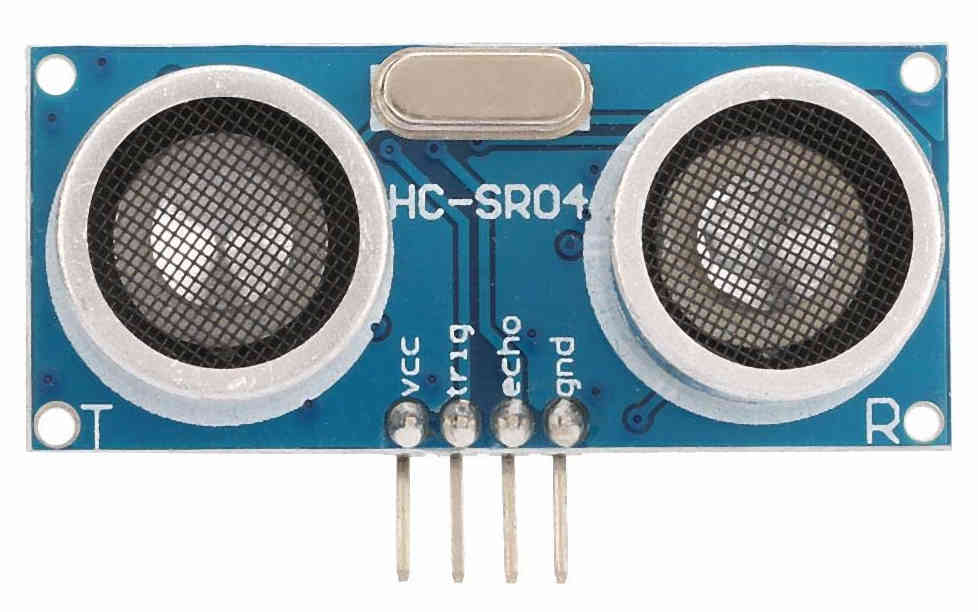
\includegraphics[width=2.0cm]{figs/hcsr04.jpg} 
\end{minipage}
\hfill
\begin{minipage}{0.3\textwidth}
    \centering
    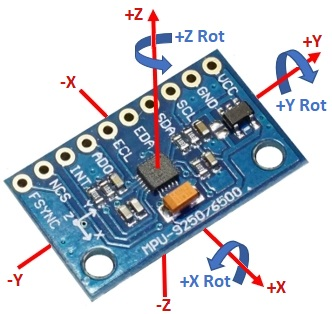
\includegraphics[width=1.8cm]{figs/mpu9250.jpg}
\end{minipage}

\vspace{-0.5cm} % Reduce el espacio entre filas

% Imagen centrada en la última fila
\begin{center}
    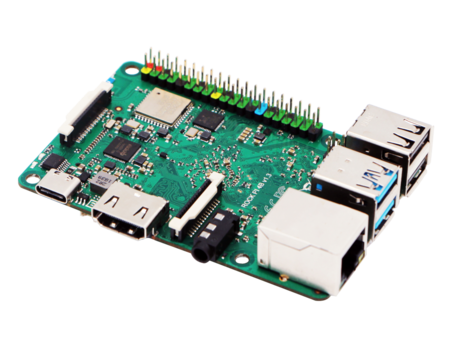
\includegraphics[width=2.7cm]{figs/raspberry4.png}
\end{center}

\end{frame}


%========= Diapositiva con matemáticas y leyenda (conditions*):
\begin{frame}
\frametitle{Software}

\centering

% Primera fila
\begin{minipage}{0.3\textwidth}
    \centering
    
\includegraphics[width=2.0cm]{figs/python.jpeg}
\end{minipage}
\hfill
\begin{minipage}{0.3\textwidth}
    \centering
    
\includegraphics[width=3.0cm]{figs/freecad.png}
\end{minipage}
\hfill
\begin{minipage}{0.3\textwidth}
    \centering
    
\includegraphics[width=2.3cm]{figs/sklearn.png}
\end{minipage}

\vspace{0.3cm} % Reduce el espacio entre filas


% Segunda fila
\begin{minipage}{0.3\textwidth}
    \centering
    
\includegraphics[width=2.3cm]{figs/librosa.png} 
\end{minipage}
\hfill
\begin{minipage}{0.3\textwidth}
    \centering
    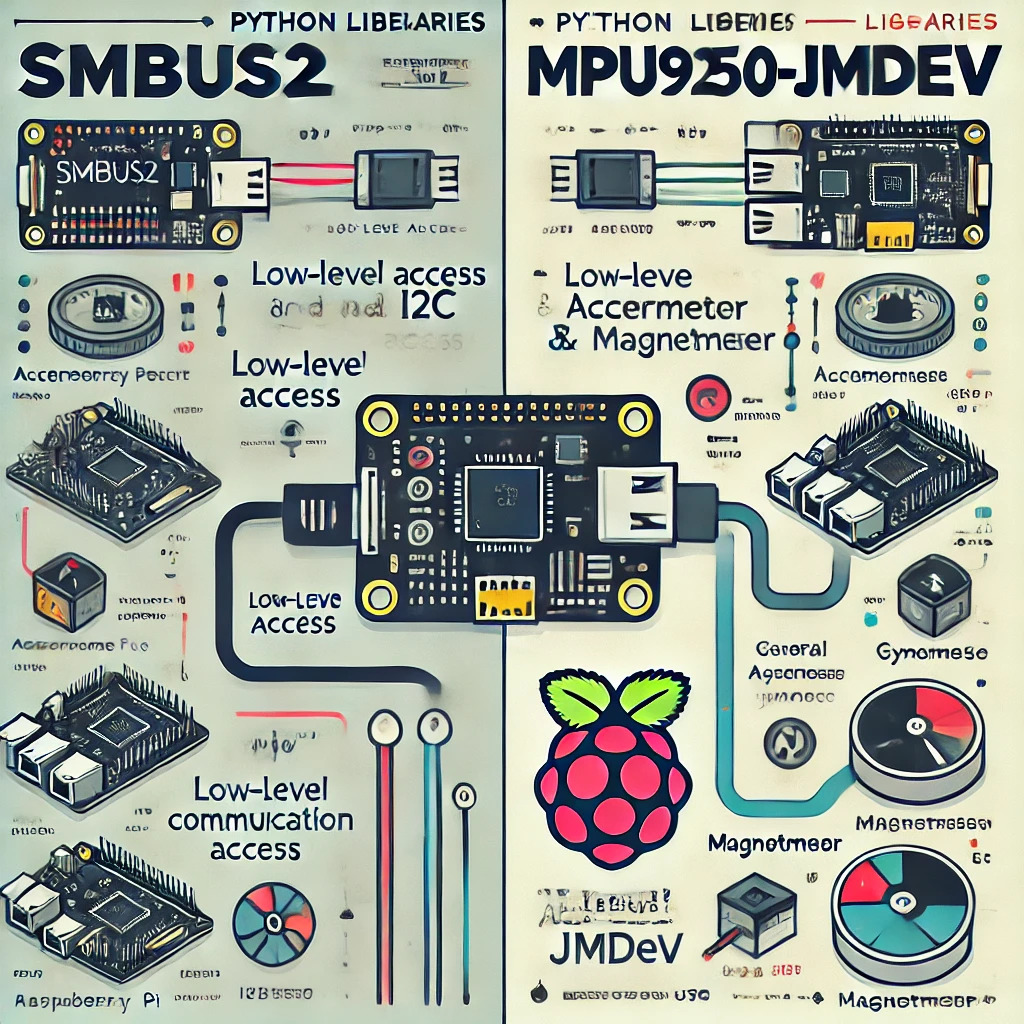
\includegraphics[width=2.0cm]{figs/mag.jpg} 
\end{minipage}
\hfill
\begin{minipage}{0.3\textwidth}
    \centering
    
\includegraphics[width=2.0cm]{figs/Jupyter.png}
\end{minipage}
% Tercera fila
\begin{minipage}{0.3\textwidth}
    \centering
    
\includegraphics[width=2.3cm]{figs/gimp.jpeg} 
\end{minipage}
\end{frame}

\section*{}
\begin{frame}{}
  \centering \Huge
  \emph{Arquitectura hardware}
\note[item]{Una vez descritos los objetivos, veamos qué hemos hecho para alcanzarlos.}
\end{frame}



\section{Arquitectura hardware}
\begin{frame}
\frametitle{Geometría del robot}
\centering
\begin{minipage}{0.45\textwidth}
    \centering
    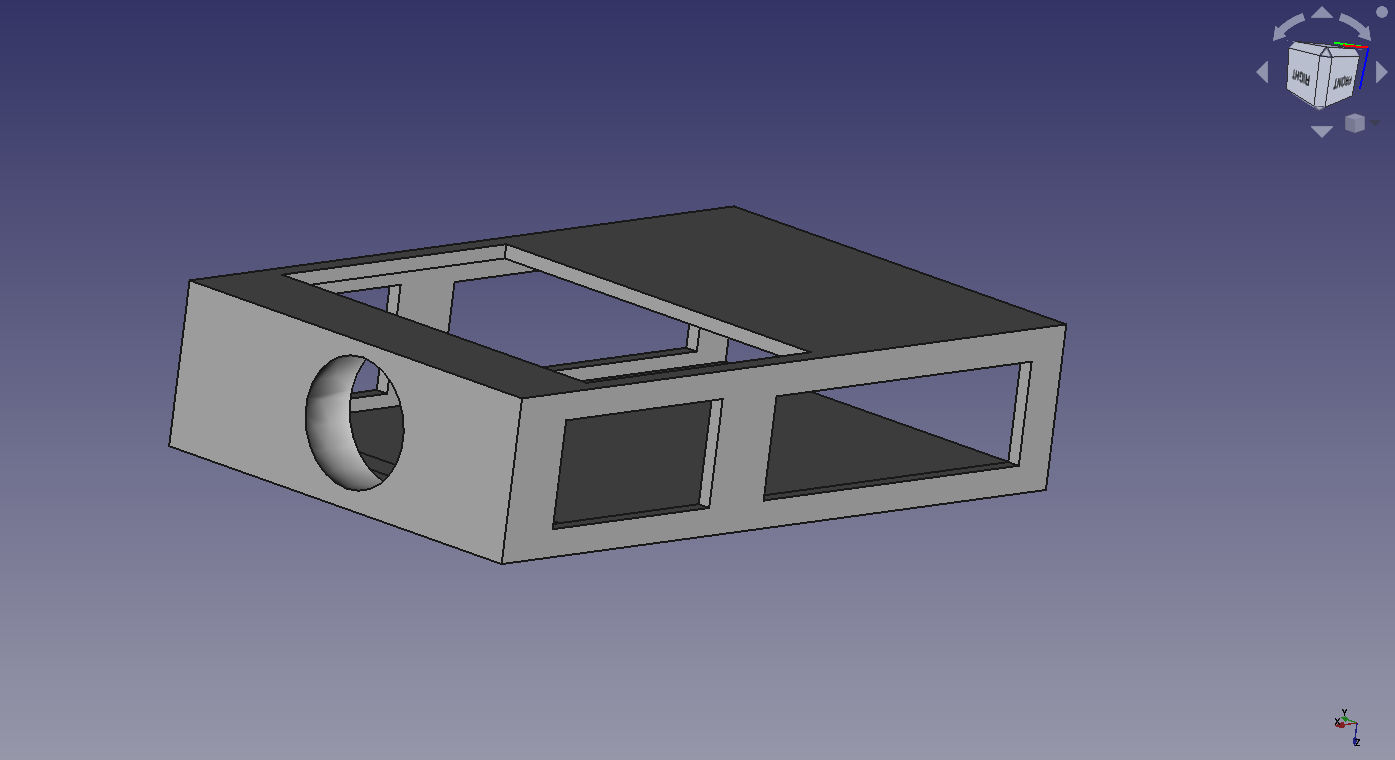
\includegraphics[width=5.8cm]{figs/base.png}
\end{minipage}
\hfill
\begin{minipage}{0.45\textwidth}
    \centering
    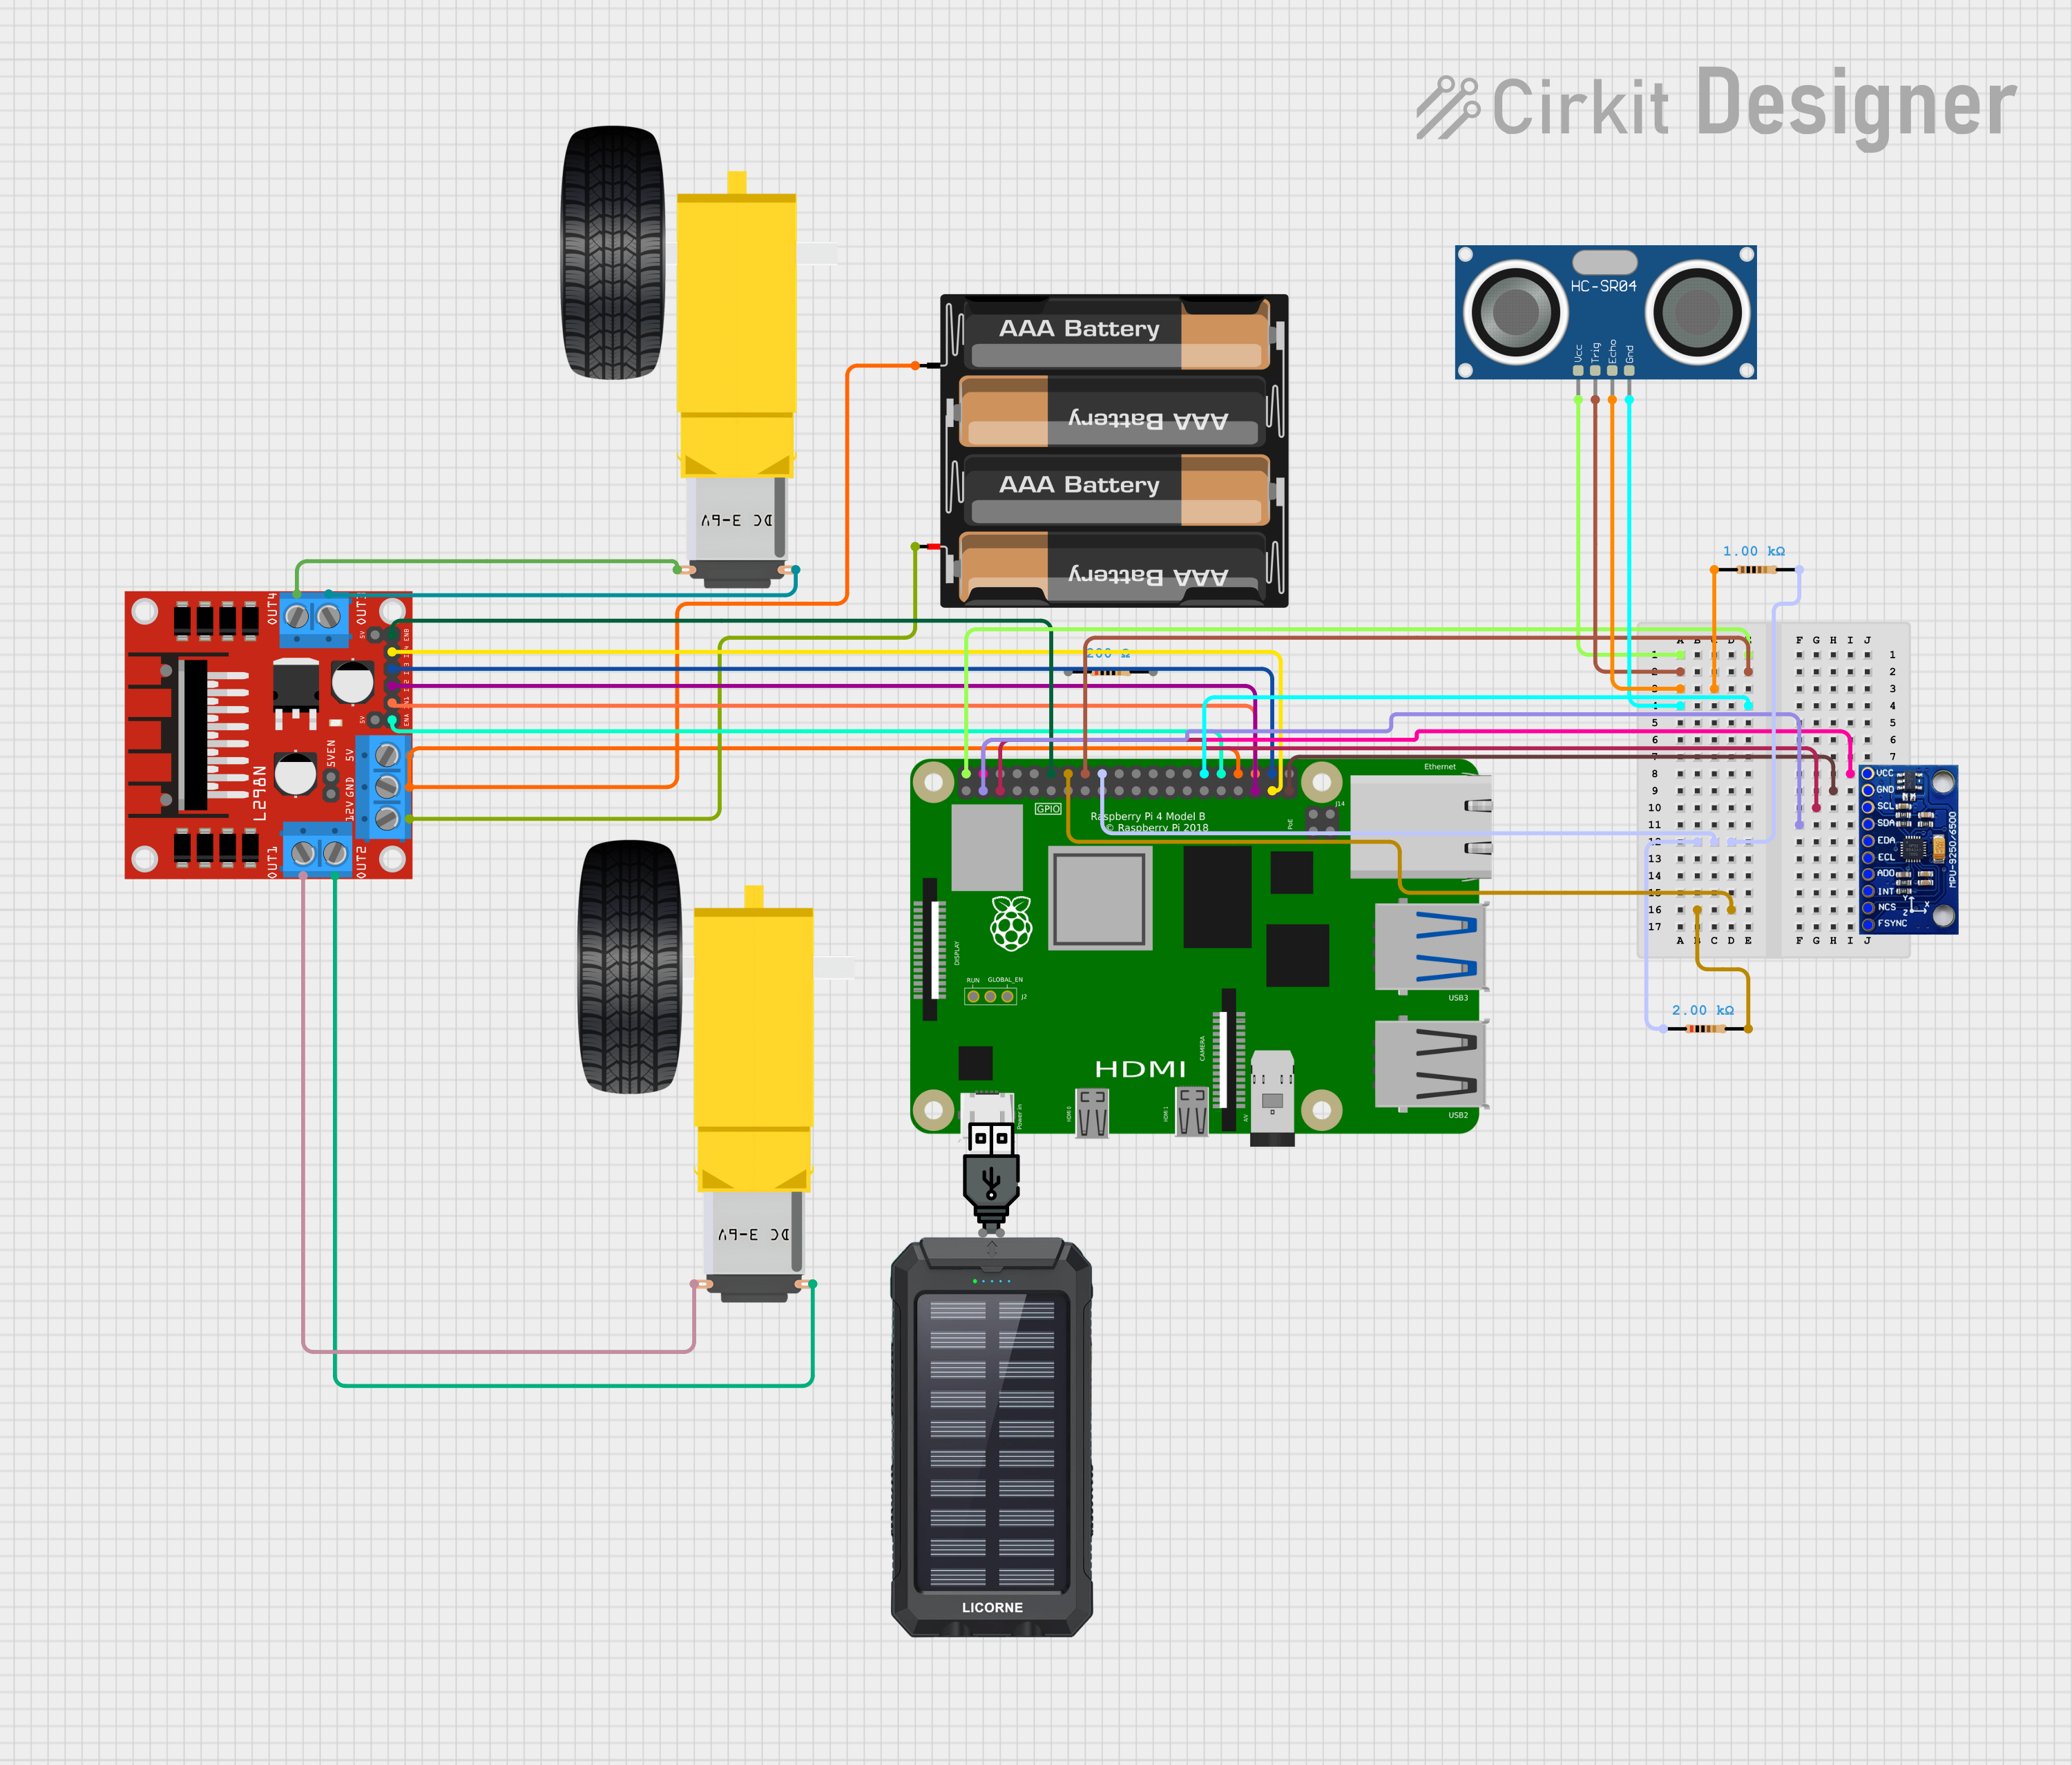
\includegraphics[width=5.5cm]{figs/final_circuito.png}
\end{minipage}

\end{frame}


\begin{frame}
\frametitle{Geometría del robot}
\centering
\begin{minipage}{0.45\textwidth}
    \centering
    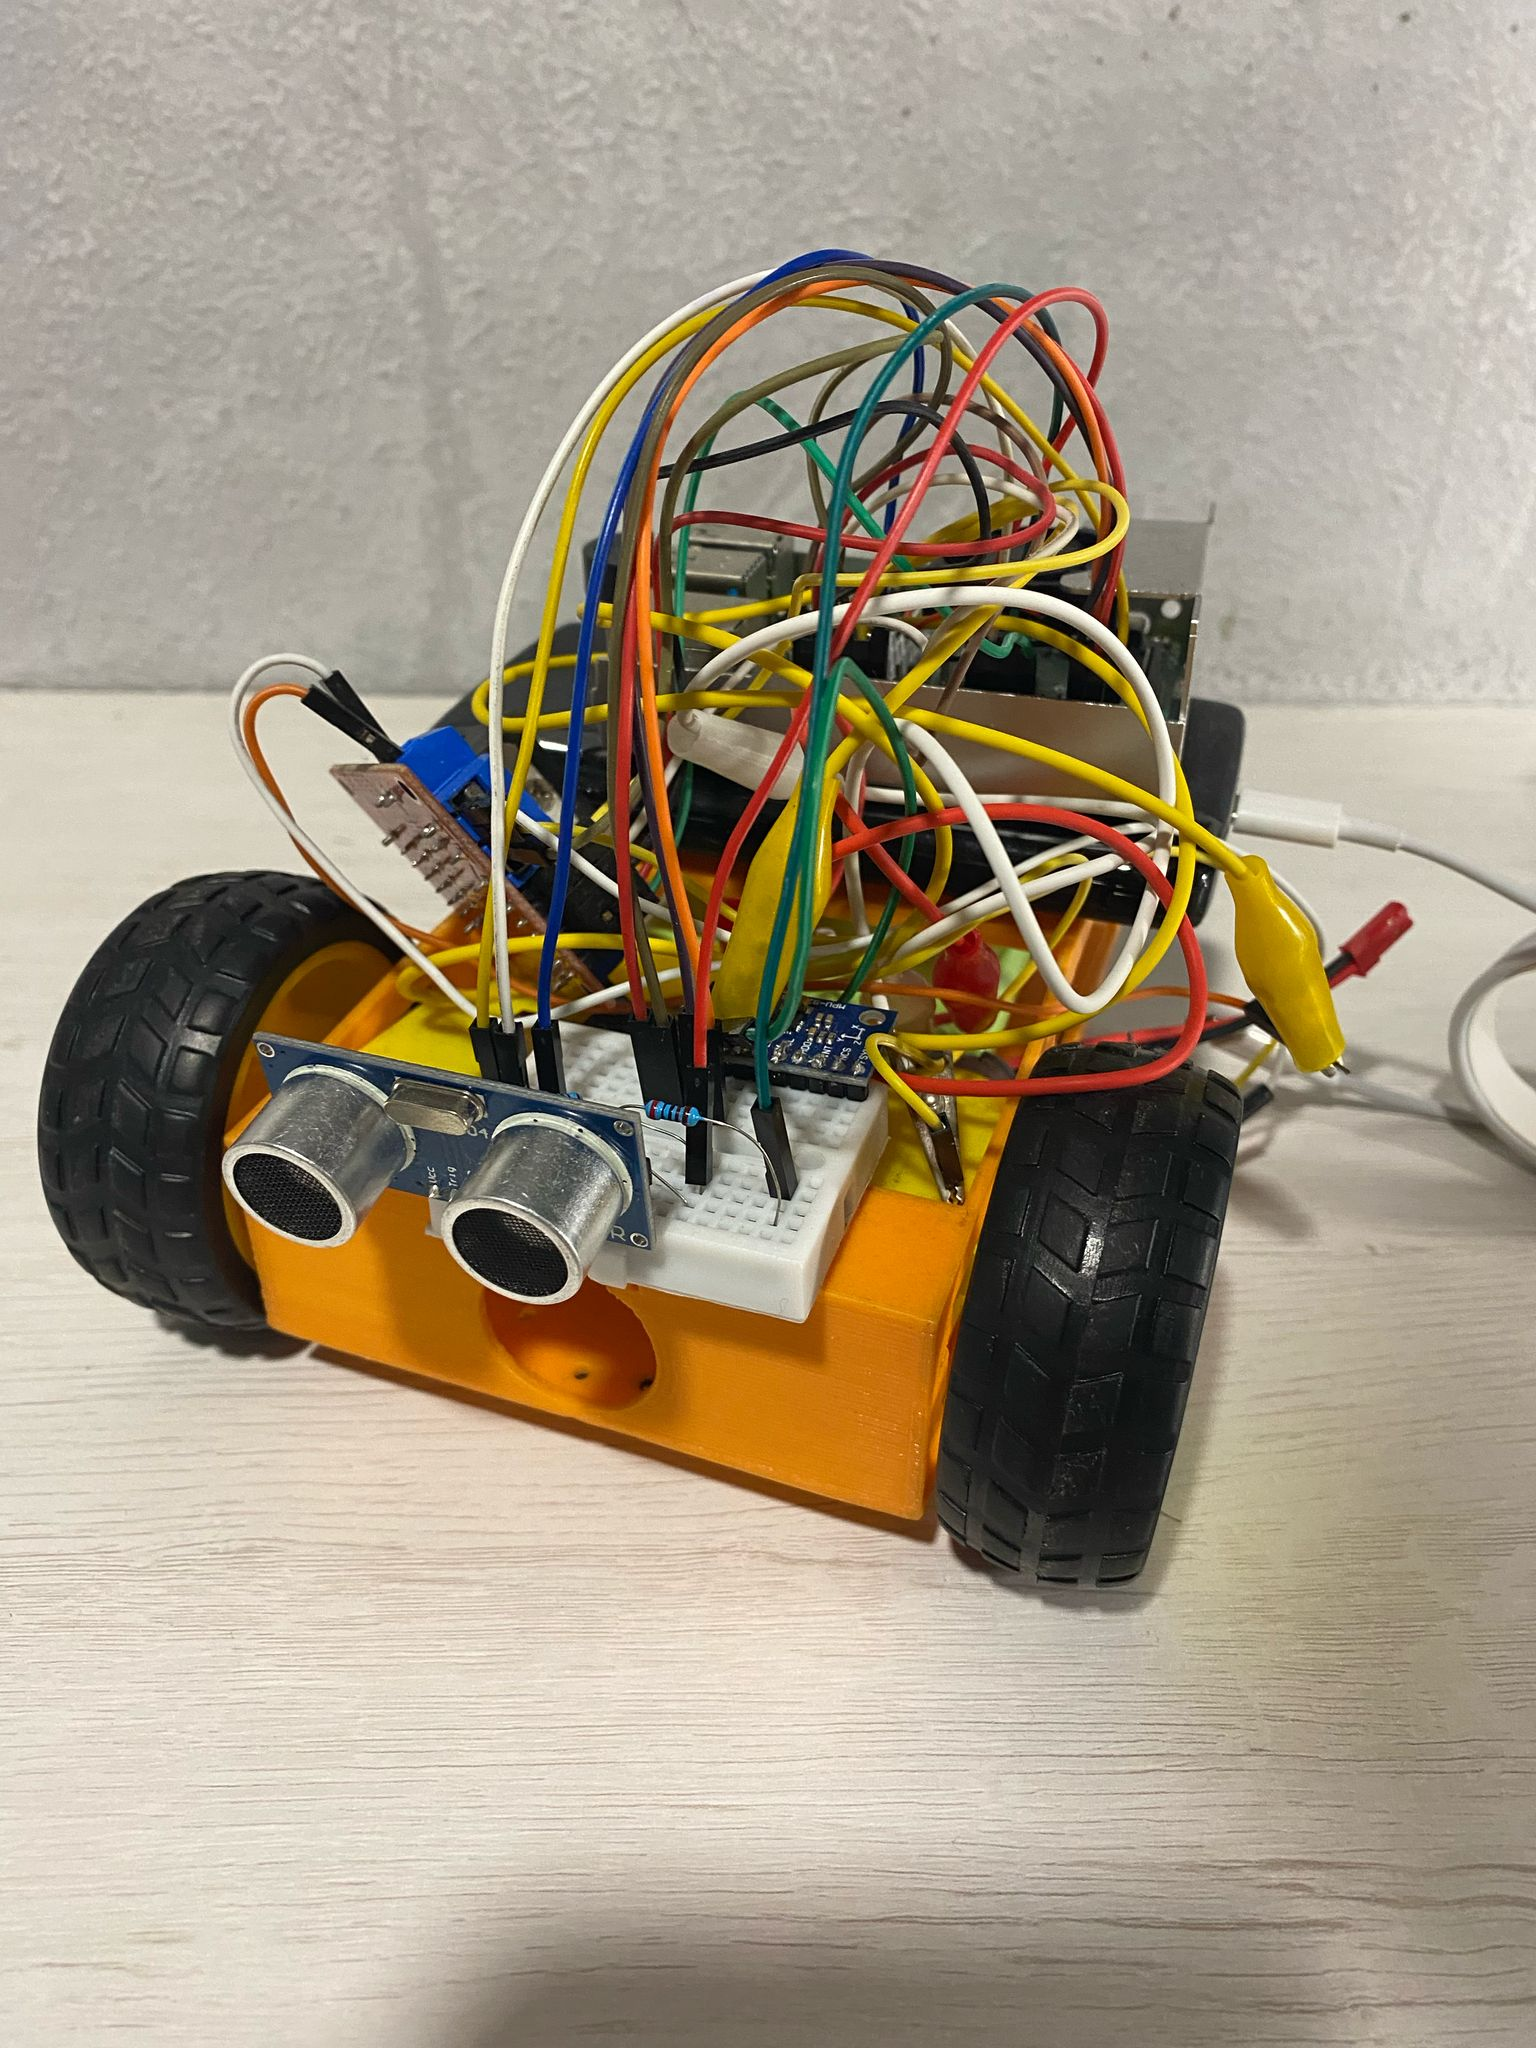
\includegraphics[width=5.4cm]{figs/rob.jpeg}
\end{minipage}


\end{frame}

\section*{}
\begin{frame}{}
  \centering \Huge
  \emph{Desarrollo software}
\end{frame}

\section{Desarrollo software}
\begin{frame}
\frametitle{Orientación y diseño del mapa}
\centering
\begin{minipage}{0.45\textwidth}
    \centering
    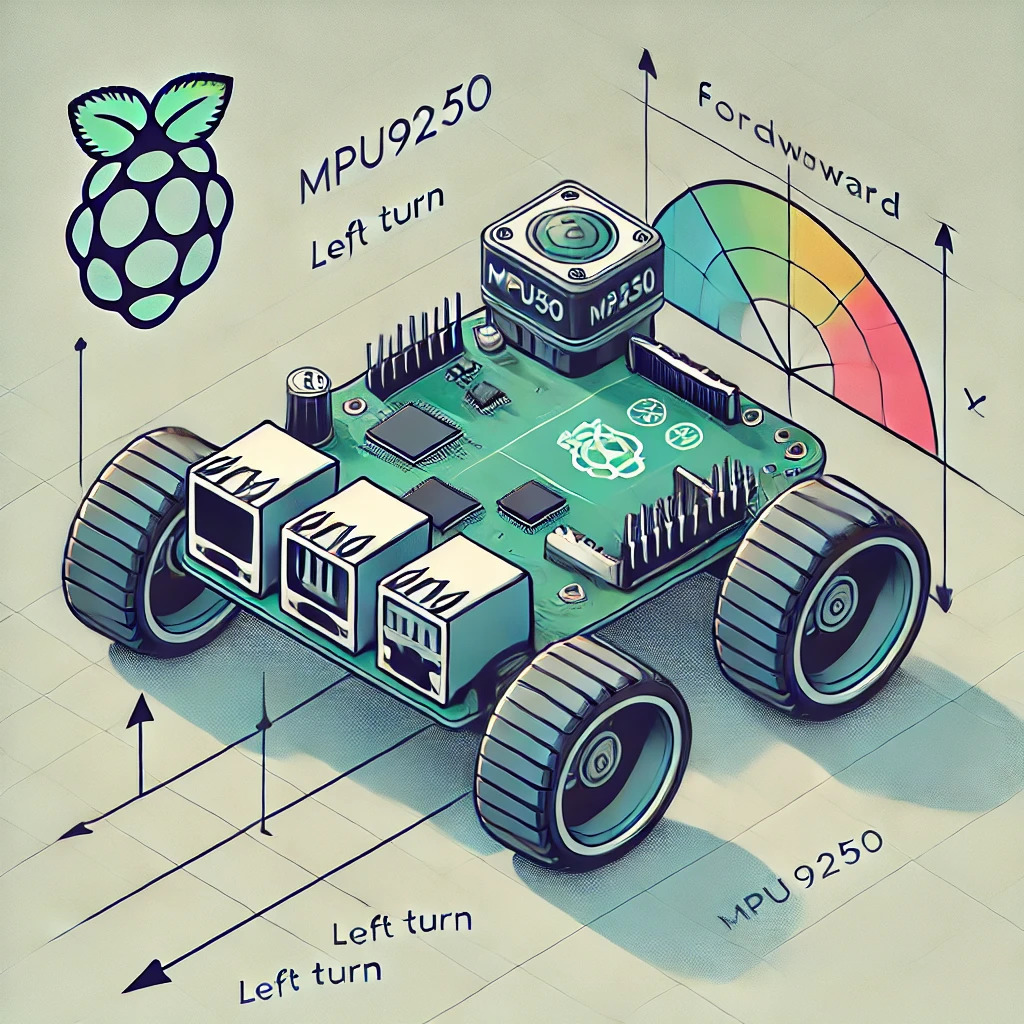
\includegraphics[width=3.6cm]{figs/pepe.jpg}
\end{minipage}
\hfill
\begin{minipage}{0.45\textwidth}
    \centering
    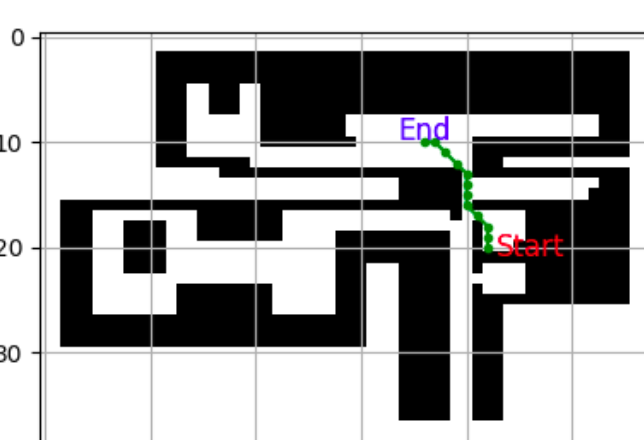
\includegraphics[width=4.5cm]{figs/path1.png}
\end{minipage}
\hfill
\vspace{0.3cm} % Reduce el espacio entre filas
\begin{minipage}{0.45\textwidth}
    \centering
    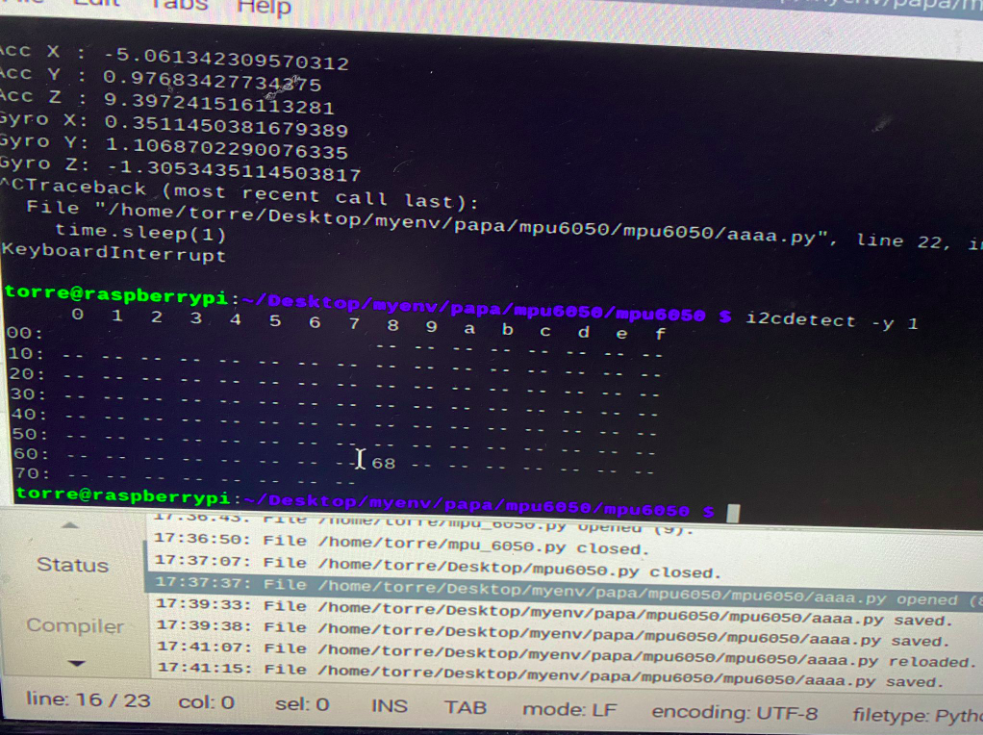
\includegraphics[width=4.5cm]{figs/bus.png}
\end{minipage}

\end{frame}


\begin{frame}
\frametitle{Interfaz de usuario}
\centering
\begin{minipage}{0.45\textwidth}
    \centering
    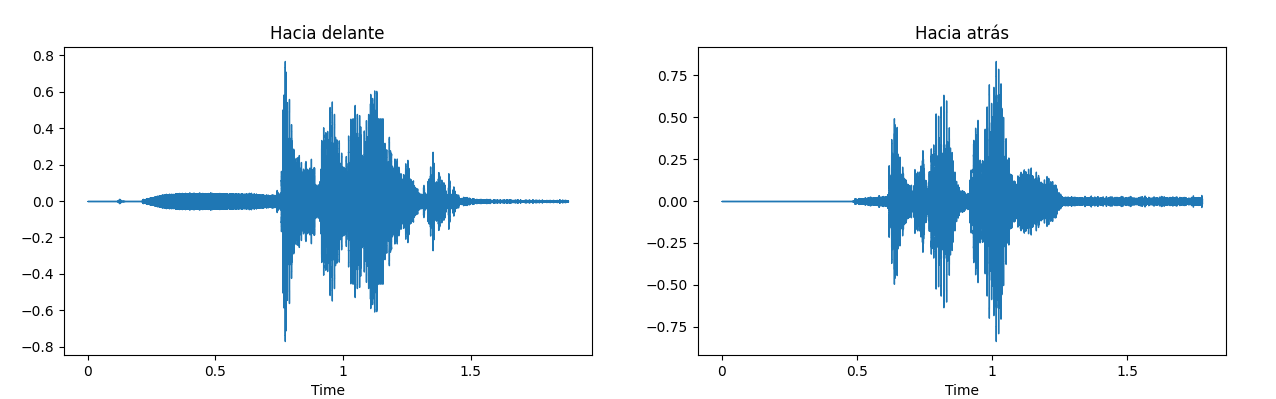
\includegraphics[width=5.5cm]{figs/forma_onda.png}
\end{minipage}
\hfill
\begin{minipage}{0.45\textwidth}
    \centering
    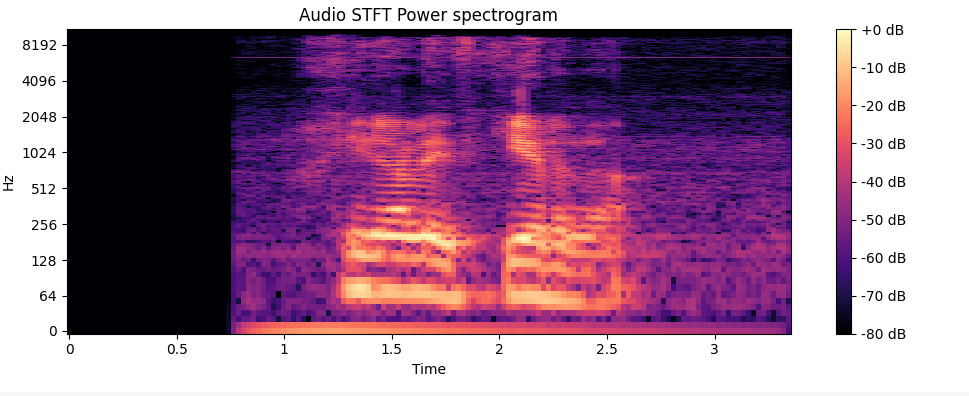
\includegraphics[width=5.5cm]{figs/stft_spectogram.png}
\end{minipage}
\hfill
\vspace{0.3cm} % Reduce el espacio entre filas
\begin{minipage}{0.45\textwidth}
    \centering
    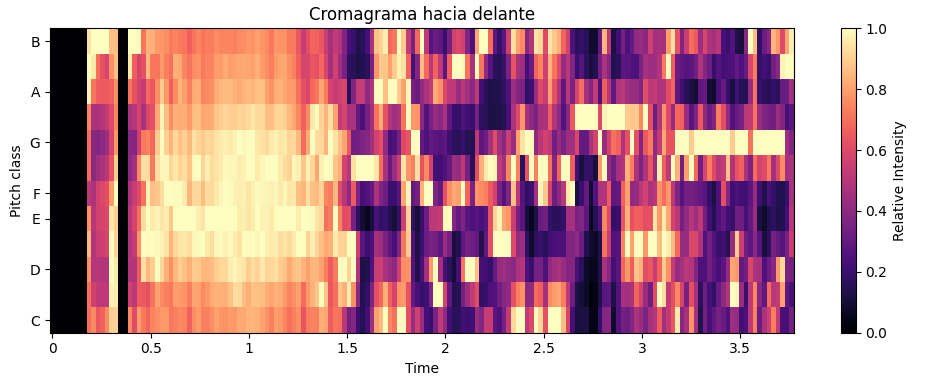
\includegraphics[width=5.5cm]{figs/cromagrama.png}
\end{minipage}
\hfill
\begin{minipage}{0.45\textwidth}
    \centering
    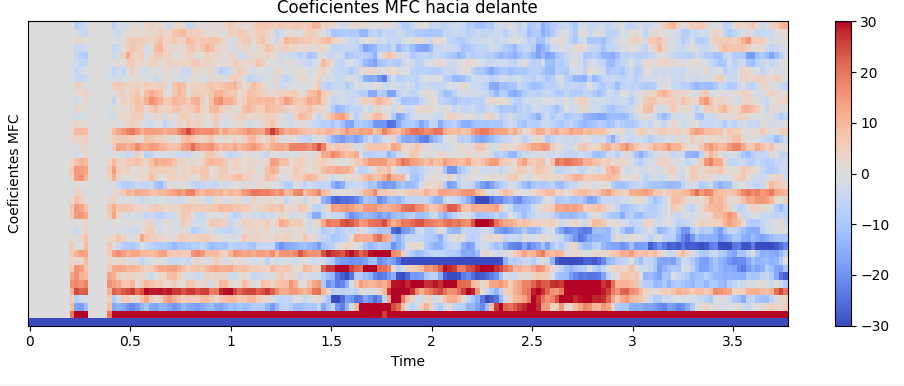
\includegraphics[width=5.5cm]{figs/coeficientes_mfc.png}
\end{minipage}
\hfill
\vspace{0.3cm} % Reduce el espacio entre filas
\begin{minipage}{0.45\textwidth}
    \centering
    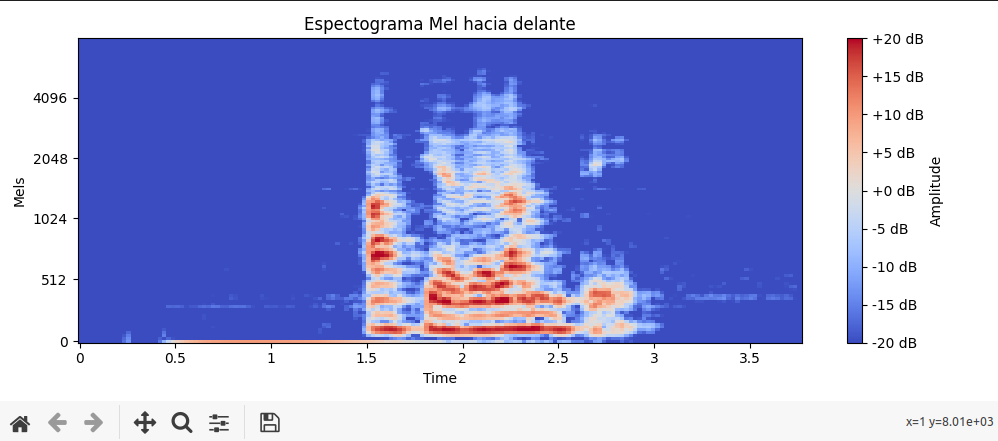
\includegraphics[width=5.5cm]{figs/mel_spectrogram.png}
\end{minipage}


\end{frame}


\begin{frame}
\frametitle{Localización}
\centering
\begin{minipage}{0.45\textwidth}
    \centering
    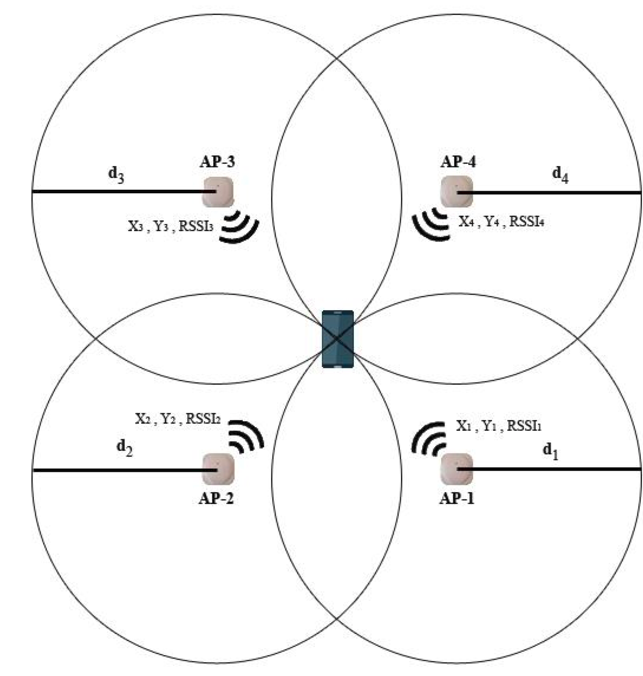
\includegraphics[width=5.5cm]{figs/trilateration.png}
\end{minipage}


\end{frame}


\begin{frame}
\frametitle{Localización}
\centering

\begin{equation}
d = 10^{\frac{A - \texttt{RSSI}}{10 \cdot n}}
\label{ec:ec2}
\end{equation}
\texttt{Donde:}
\begin{itemize}
    \item $d$: Distancia estimada en metros.
    \item $A$: Valor RSSI a 1 metro del AP.
    \item \texttt{RSSI}: Potencia recibida.
    \item $n$: Factor de propagación.
\end{itemize}
\vspace{0.3cm} % Reduce el espacio entre filas
\begin{equation}
\left\{
	\begin{array}{lcc}
		(x - x_1)^2 + (y - y_1)^2 = (d_1)^2\\
		(x - x_2)^2 + (y - y_2)^2 = (d_2)^2\\
		(x - x_3)^2 + (y - y_3)^2 = (d_3)^2 \\
		(x - x_4)^2 + (y - y_4)^2 = (d_4)^2
	\end{array}
\right.
\label{ec:ec5}
\end{equation}

\end{frame}


\begin{frame}
\frametitle{Navegación (A*)}
\centering


\begin{minipage}{0.45\textwidth}
    \centering
    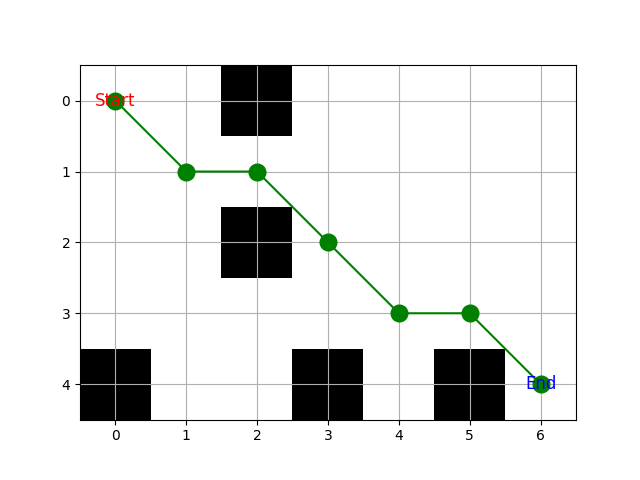
\includegraphics[width=5.5cm]{figs/astar4.png}
\end{minipage}

\vspace{-0.6cm} % Reduce el espacio entre filas
\begin{equation}
\left\{
	f(n) = g(n) + h(n)
\right.
\label{ec:ec678}
\end{equation}

\texttt{Donde:}
\begin{itemize}
    \item $g(n)$: Coste de cada movimiento.
    \item $h(n)$: Heurística.
\end{itemize}

\end{frame}

\section*{}
\begin{frame}{}
  \centering \Huge
  \emph{Pruebas y experimentos}
\end{frame}


\section{Pruebas y experimentos}
\begin{frame}
\frametitle{Calibración magnética}
\centering

% Primera fila
\begin{minipage}{0.45\textwidth}
    \centering
    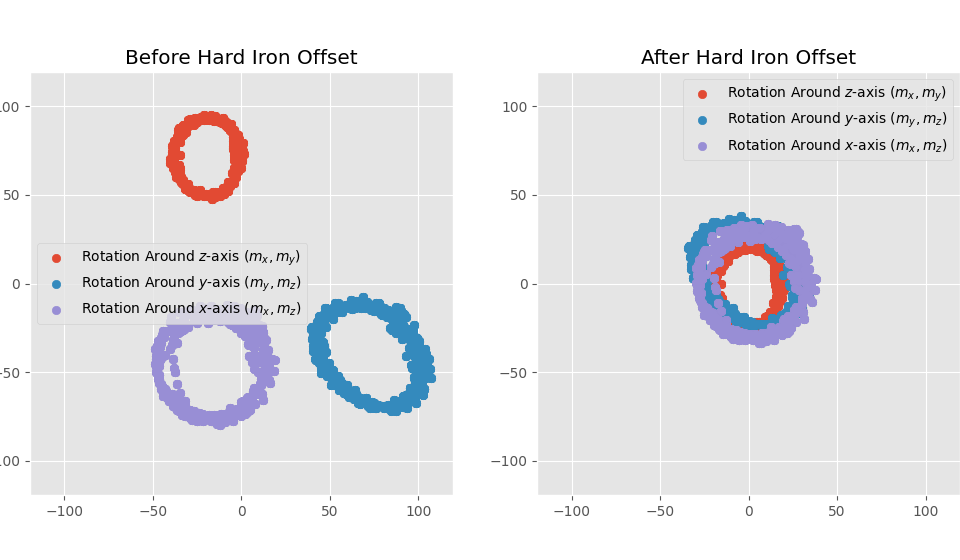
\includegraphics[width=6.5cm]{figs/hard_iron_calibration.png}
\end{minipage}
\hfill
\begin{minipage}{0.45\textwidth}
    \centering
    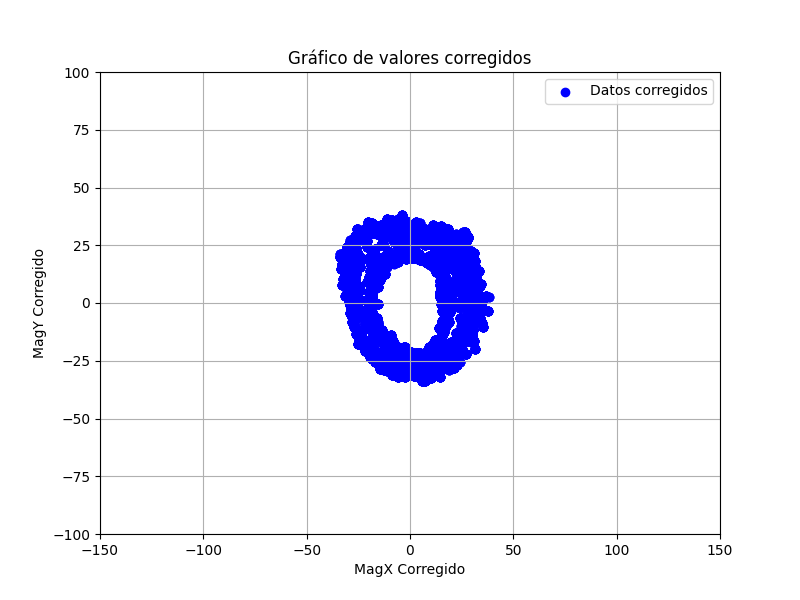
\includegraphics[width=5.0cm]{figs/soft_iron_calibration.png}
\end{minipage}

\vspace{0.5cm} % Espacio entre filas

% Segunda fila
\begin{minipage}{0.7\textwidth}
    \centering
    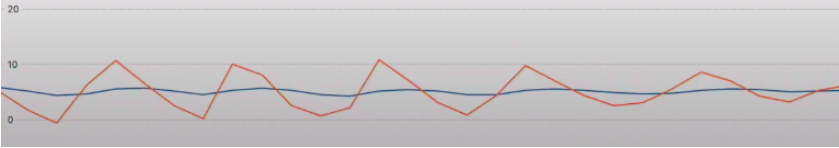
\includegraphics[width=8.0cm]{figs/low.png} % Cambia por la ruta de la tercera imagen
\end{minipage}
\hfill


\end{frame}



\begin{frame}
\frametitle{Elección del modelo de aprendizaje automático}
\centering

\centering

\begin{table}[H]
\begin{center}
\begin{tabular}{|c|c|c|c|c|}
\hline
\textbf{Classifier} & \textbf{Accuracy Score}\\
\hline
KNeighborsClassifier & 93.75\%  \\  
SVC & 100.00\%  \\
SVC RBF kernel & 93.75\%  \\
DecisionTreeClassifier & 87.50\%  \\
RandomForestClassifier & 100.00\%  \\
AdaBoostClassifier & 43.75\%  \\
GaussianNB & 93.75\%  \\
QuadraticDiscriminantAnalysis & 31.25\  \\
MLPClassifier & 93.75\%  \\
\hline
\end{tabular}
\label{cuadro:tabla2}
\end{center}
\end{table}

\end{frame}


\begin{frame}
\frametitle{Elección del número de APs}
\centering

% Primera fila
\begin{minipage}{0.45\textwidth}
    \centering
    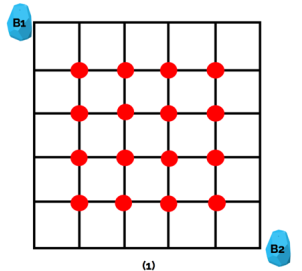
\includegraphics[width=4.0cm]{figs/dos_apes.png}
\end{minipage}
\hfill
\begin{minipage}{0.45\textwidth}
    \centering
    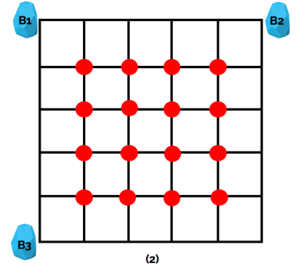
\includegraphics[width=4.0cm]{figs/tres_apes.png}
\end{minipage}

\vspace{0.3cm} % Espacio entre filas

% Segunda fila
\begin{minipage}{0.45\textwidth}
    \centering
    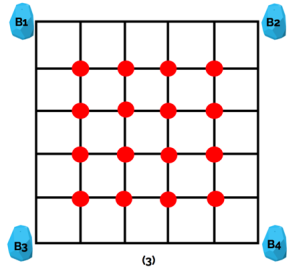
\includegraphics[width=4.0cm]{figs/cuatro_apes.png} % Cambia por la ruta de la tercera imagen
\end{minipage}
\hfill
\begin{minipage}{0.45\textwidth}
    \centering
    \includegraphics[width=4.0cm]{figs/cuatro_apes_espaciados.png} % Cambia por la ruta de la cuarta imagen
\end{minipage}

\end{frame}



\begin{frame}
\frametitle{Elección del número de APs}
\centering

\begin{table}[H]
\begin{center}
\begin{tabular}{|c|c|c|c|c|}
\hline
\textbf{Nodos} & \textbf{SVC, Linear} & \textbf{SVC,RBF} & \textbf{DTREE} & \textbf{RF} \\
\hline
2 & 28\% & 31\% & 28\% & 24\% \\  
3 & 82\% & 86\% & 78\% & 82\% \\   
4 & 94\% & 94\% & 91\% & 94\% \\   
\hline
\end{tabular}
\label{cuadro:tabla2}
\end{center}
\end{table}

\begin{table}[H]
\begin{center}
\begin{tabular}{|c|c|c|c|c|}
\hline
\textbf{Nodos} & \textbf{SVC, Linear} & \textbf{SVC,RBF} & \textbf{DTREE} & \textbf{RF} \\
\hline
4 & 99\% & 99\% & 96\% & 100\% \\  
\hline
\end{tabular}
\label{cuadro:tabla3}
\end{center}
\end{table}

% Primera fila
\begin{minipage}{0.45\textwidth}
    \centering
    \includegraphics[width=5.2cm]{figs/vals1.png}
\end{minipage}
\hfill
\begin{minipage}{0.45\textwidth}
    \centering
    \includegraphics[width=5.2cm]{figs/vals2.png}
\end{minipage}

\vspace{0.3cm} % Espacio entre filas
\end{frame}




\section*{}
\begin{frame}{}
  \centering \Huge
  \emph{Conclusiones}
\end{frame}


\section{Conclusiones}
\begin{frame}
\begin{block}{Objetivos cumplidos}
\begin{itemize}
\item Robot móvil de bajo coste.
\item CPU de baja capacidad de cómputo.
\item Navegación, orientación y localización en interiores.
\item Portabilidad.
\item Comunicación.
\end{itemize}

\begin{itemize}
\item \href{https://youtube.com/shorts/wm4-3SVO6g4?feature=share}{https://youtube.com/shorts/wm4-3SVO6g4?feature=share}
\item \href{https://youtube.com/shorts/i80oPc5RJ9w?feature=share}{https://youtube.com/shorts/i80oPc5RJ9w?feature=share}
\end{itemize} 

\end{block}

\end{frame}



\begin{frame}
\begin{block}{Líneas futuras}
\begin{itemize}
\item Aumentar datos de entrenamiento.
\item Smartphones.
\item Áreas de mayor tamaño y más dispositivos Wi-Fi.
\item Altavoz.
\item Nuevas rutas.
\end{itemize}
\end{block}
\end{frame}

\begin{frame}[plain]
\large{\titlepage}
\note[item]{Y hasta aquí mi exposición.}
\note[item]{Quedo a disposición del tribunal...}
\end{frame}


\end{document}
